
% ibs.tex

\documentclass[10pt,a4paper,titlepage]{article}
\usepackage[czech]{babel}
\usepackage[utf8]{inputenc}
\usepackage[margin=100pt]{geometry}
    
\usepackage{graphicx}   % Import pictures
\usepackage{multicol}
\usepackage{caption}
\usepackage{subcaption}
%\usepackage{csquotes}

\usepackage[backend=biber, sorting=none]{biblatex}
\addbibresource{ibs.bib}
    
\begin{document}
  \pagenumbering{gobble}

  \begin{center}
    \section*{Analýza aplikačního protokolu zabezpečeného SSL/TLS}
    Martin Beneš
  \end{center}

  \section*{Úvod}
  SSL/TLS jsou protokoly, řešící důvěrnost komunikace typu klient-server pomocí šifrování.
  Zajišťují také autentizaci, integritu a nepopiratelnost. Pracují mezi aplikační a
  transportní vrstvou, vyžadují spolehlivý přenost, tedy většinou na TCP, umožňují šifrovat
  komunikaci existujících aplikačních protokolů (email - SMTP, www - HTTP).
  Vyžadují autentizaci serveru (pomocí certifikátu) klientem, nepovinně také vice versa
  klienta serveru. \cite{DigiCert} \cite{RootSsl}

  TLS navazuje na SSL protokol, po SSL 3.0 z roku 1996 vyšel v roce 1999 TLS 1.0.
  Fakticky jsou si velmi podobné, SSL 3.0 (dokonce i TLS 1.0) je dnes považován obecně
  za nezabezpečený, je možné jej prolomit BEAST útokem. Novější verze TLS se snaží
  odstraňovat chyby a zamezovat útokem, a jsou považovány za marginálně bezpečnější.
  \cite{LuxSci}

  \subsection*{Princip}
  Příchozí požadavek na server musí nejprve udělat tzv. SSL handshake, při kterém je
  nutné se autentizovat a vyměnit si klíč pro symetrické šifrování dat. Úplný počátek
  komunikace je nešifrovaná, jelikož odesilatel zná pouze adresátovu adresu (IP, popř.
  DNS, kterou převede na IP), tedy ani veřejný klíč, kterým by mohl šifrovat.
  Záhy přechází na asymetrické šifrování. Využívá se zde nejčastěji RSA, DSA,
  Diffie-Hellman, nebo Fortezza.

  \begin{figure}[h!]
    \begin{center}
      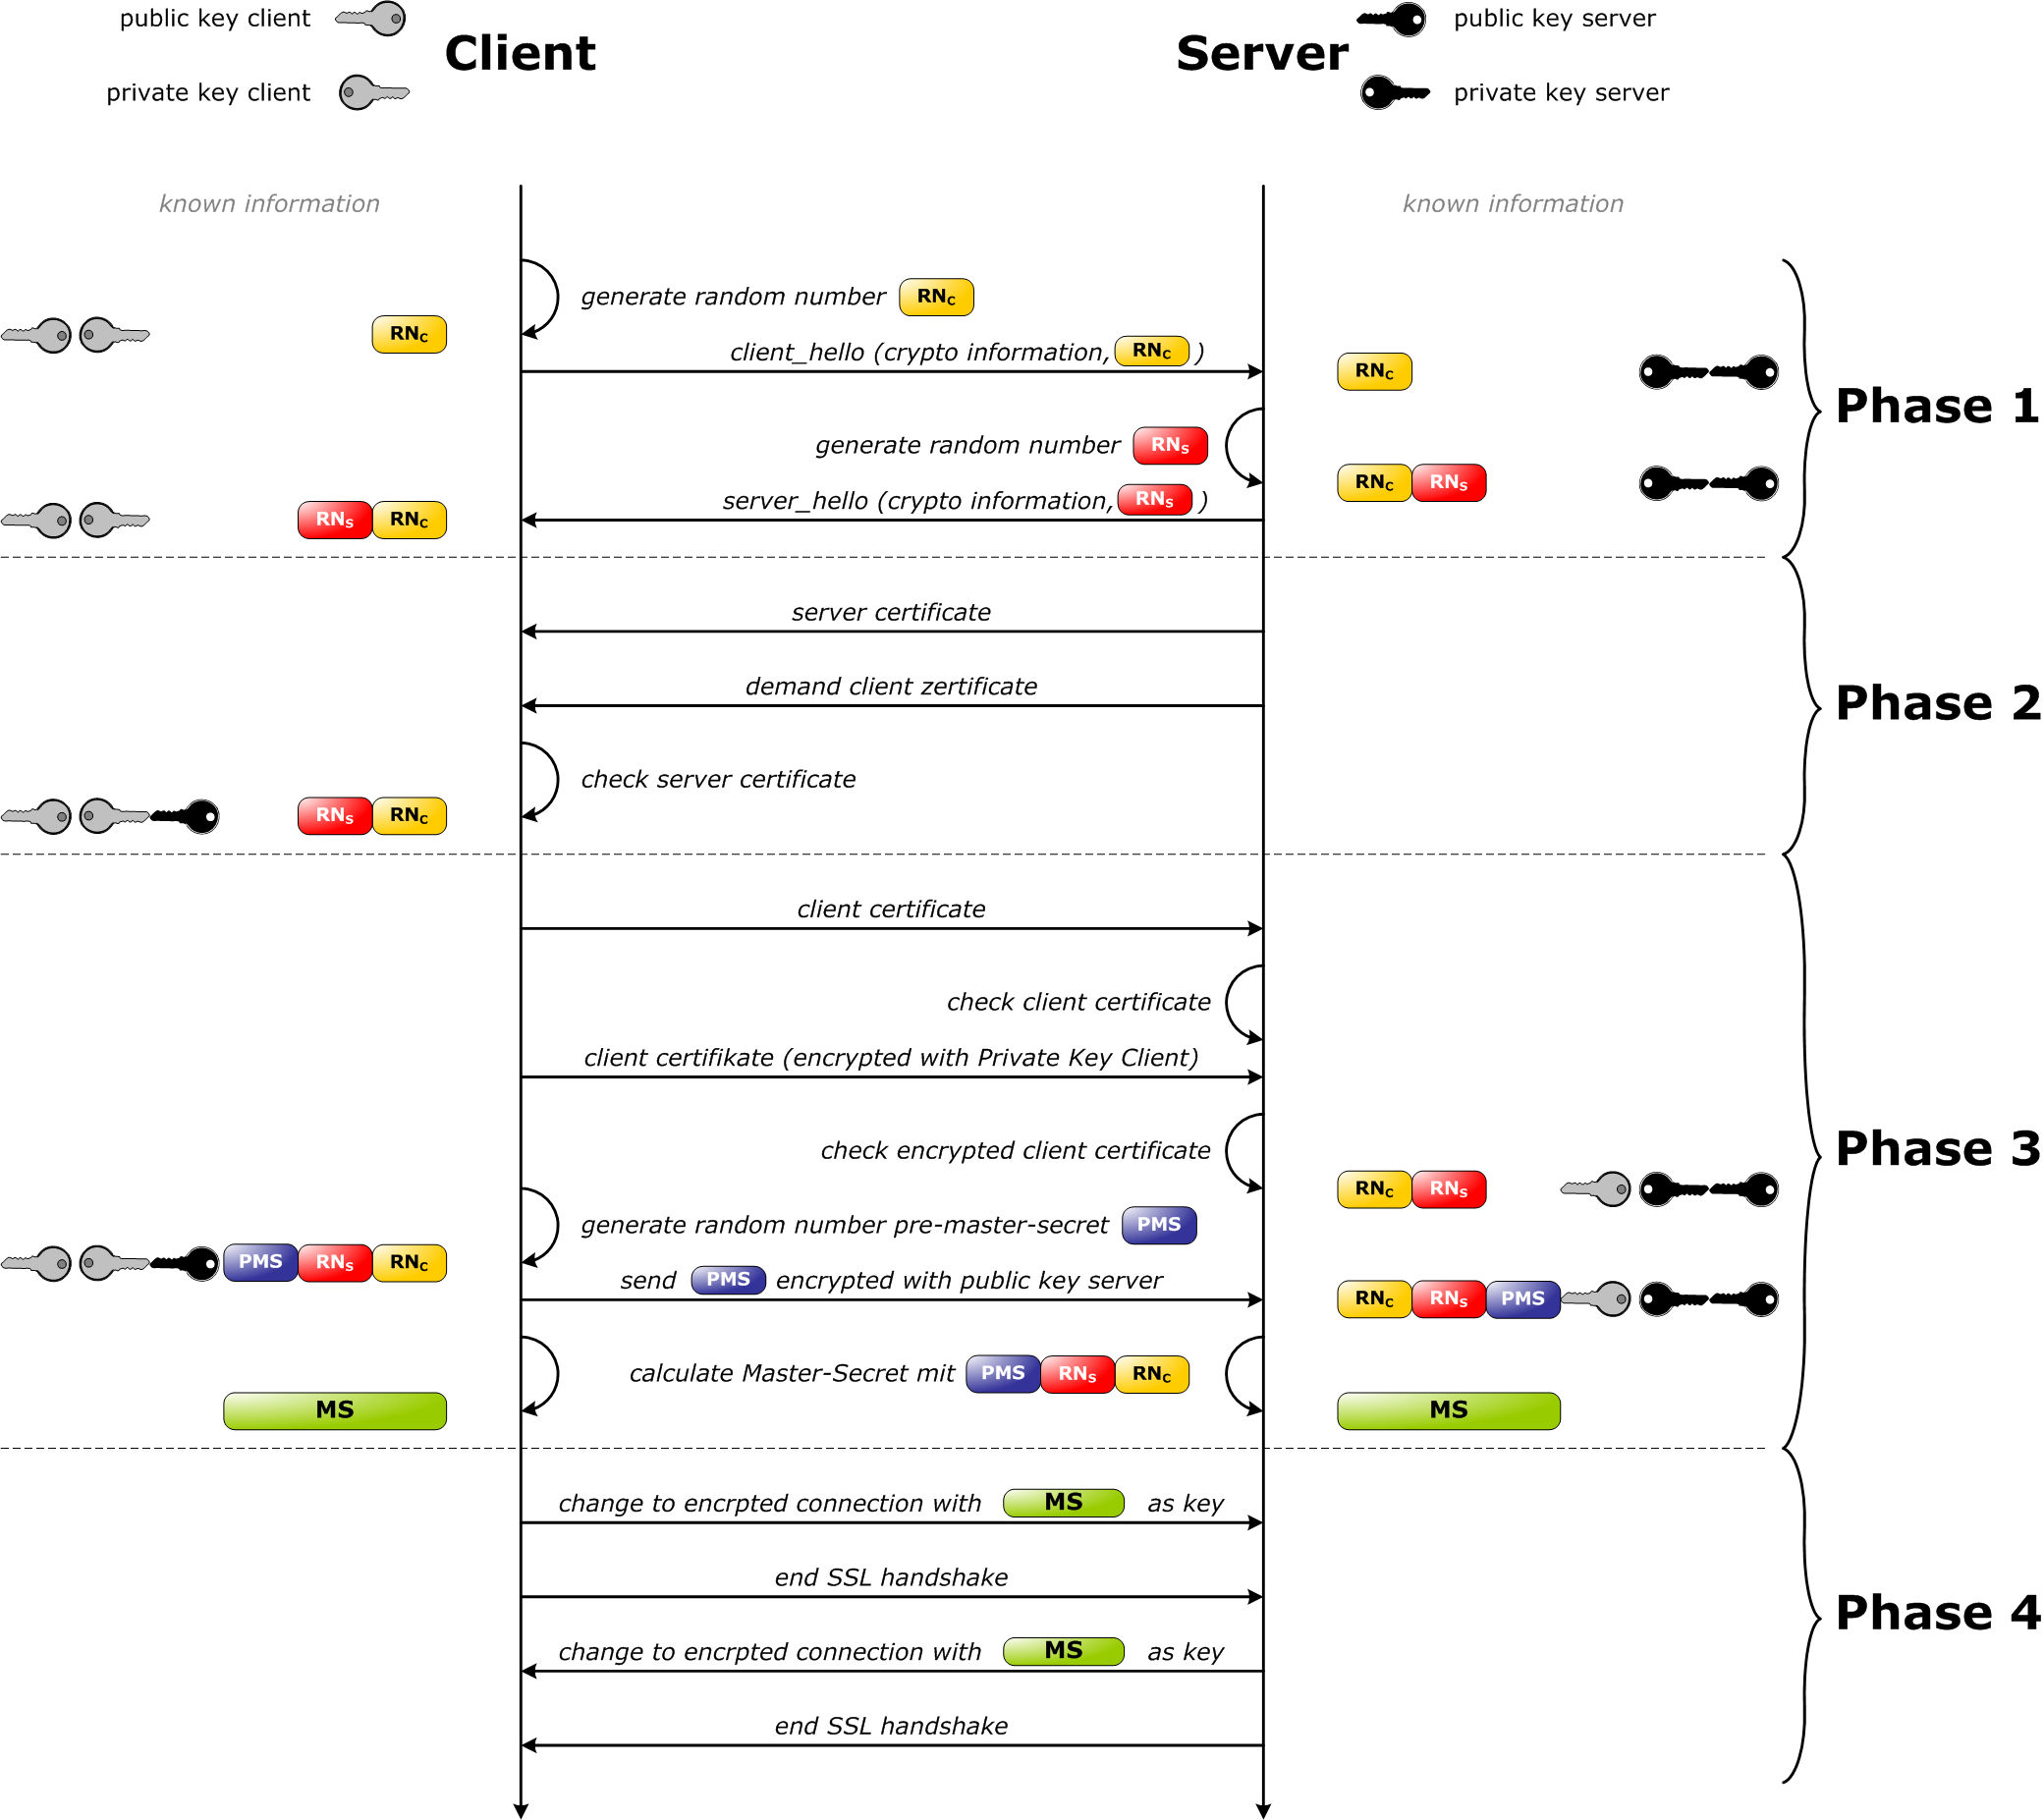
\includegraphics[width=0.6\textwidth]{ssl.png}
      \caption{Schéma SSL handshake\label{fig:sslhandshake} \cite{WikiSSL}}
    \end{center}    
  \end{figure}

  Následně je možné již odesílat data šifrovaná symetricky klíčem, který si vyměnily
  strany při handshake fázi. Používými algoritmy jsou RC2, RC4, IDEA, DES, 3DES nebo AES.
  Pro zajištění integrity se využívají hashovací funkce, nejčastěji MD5, nebo SHA.

  \subsection*{Zranitelnosti}
  Na SSL/TLS protokoly je popsáno několik možností útoků. Dvěma nejznámějšími
  jsou SSL Beast a SSL/TLS renegotiation.
  
  \paragraph{SSL Beast}
  SSL Beast je útok na straně klienta, založen na dešifrování tajné zprávy.
  Funguje na SSL a TLS 1.0, zabezpečenými blokovou šifrou (AES, DES), na proudové
  šifry je neúčinný. \cite{sslbeast}

  \paragraph{SSL/TLS renegotiation}
  SSL/TLS renegotiation (znovuvyjednání) je útok nad SSL/TLS na principu MITM.
  Uplatňuje se v průběhu SSL/TLS handshake fáze. Je funkční na SSL 3.0 a TLS.
  Útočník naruší obsah zprávy, je schopen zasílat příkazy serveru (např. HTTP),
  který je zpracovává jako od legitimního klienta. \cite{sslrenegotiation}

  
  \section*{Realizace útoku}

  Šifrování je založené na jednoduché premise, že případná třetí strana, která nemá
  znát obsah komunikace, nezná klíč, a tudíž není schopná komunikaci číst.
  Při znalosti klíče je ale samozřejmě jednoduché rozšifrovat komunikaci. To je možné
  provést na konkrétní stanici. V operačním systému lze nastavit, aby internetové
  prohlížeče (např. Google Chrome, Mozzila Firefox) veškerá hesla pro komunikaci 
  šifrovanou pomocí SSL/TLS ukládaly do konkrétního souboru (ve Windows
  se řídí obsahem proměnné prostředí {\it SSLKEYLOGFILE}), který je možné změnit
  v ovládacích panelech, pokud má daný uživatel správcovská práva). Ukázkový
  obsah souboru je možné vidět na obrázku \ref{fig:sslkeylog}.

  \begin{figure}[h!]
    \begin{center}
      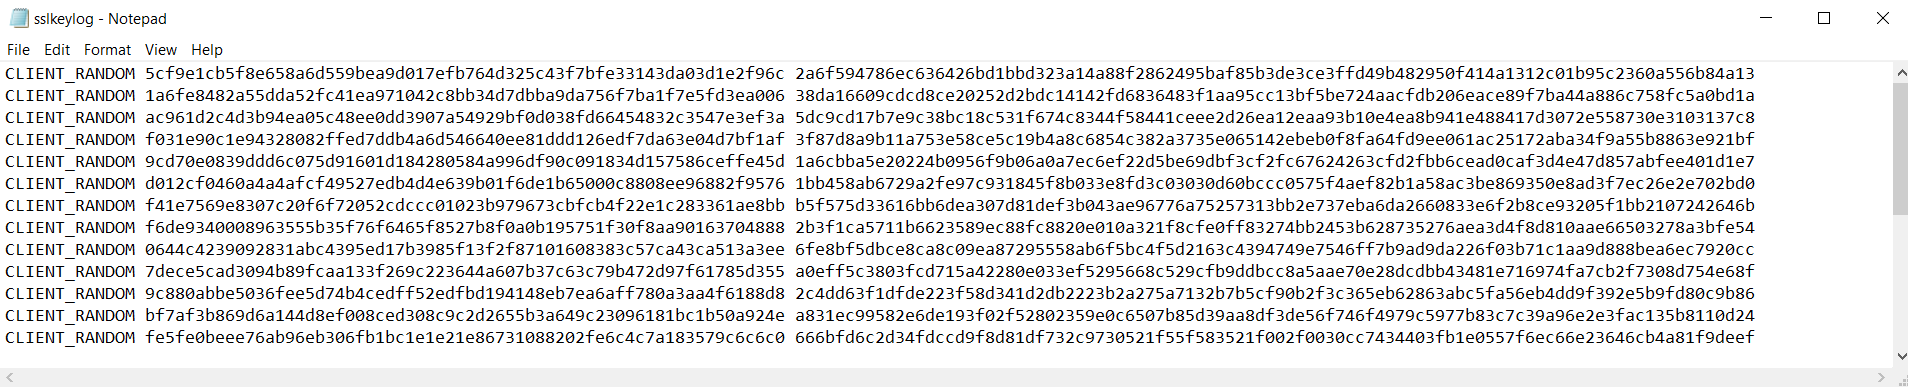
\includegraphics[width=0.9\textwidth]{sslkeylog.png}
      \caption{Obsah souboru s SSL/TLS klíči.\label{fig:sslkeylog}}
    \end{center}    
  \end{figure}
  
  Následně je nutné zadat Wiresharku, kde má pro SSL hledat klíče. Poté již stačí
  pasivně odposlouchávat komunikaci ({\it eavesdropping}) a Wireshark si při zachyceném
  SSL/TLS handshake sám spojí nově získané klíče s komunikací a při následném zachytávání
  šifrované komunikace již zná klíč i použitý algoritmus a přímo zobrazuje dešifrovaná
  data (např HTTP2), jak je zobrazeno na obrázku \ref{fig:decrypted}.

  \begin{figure}[h!]
    \begin{center}
      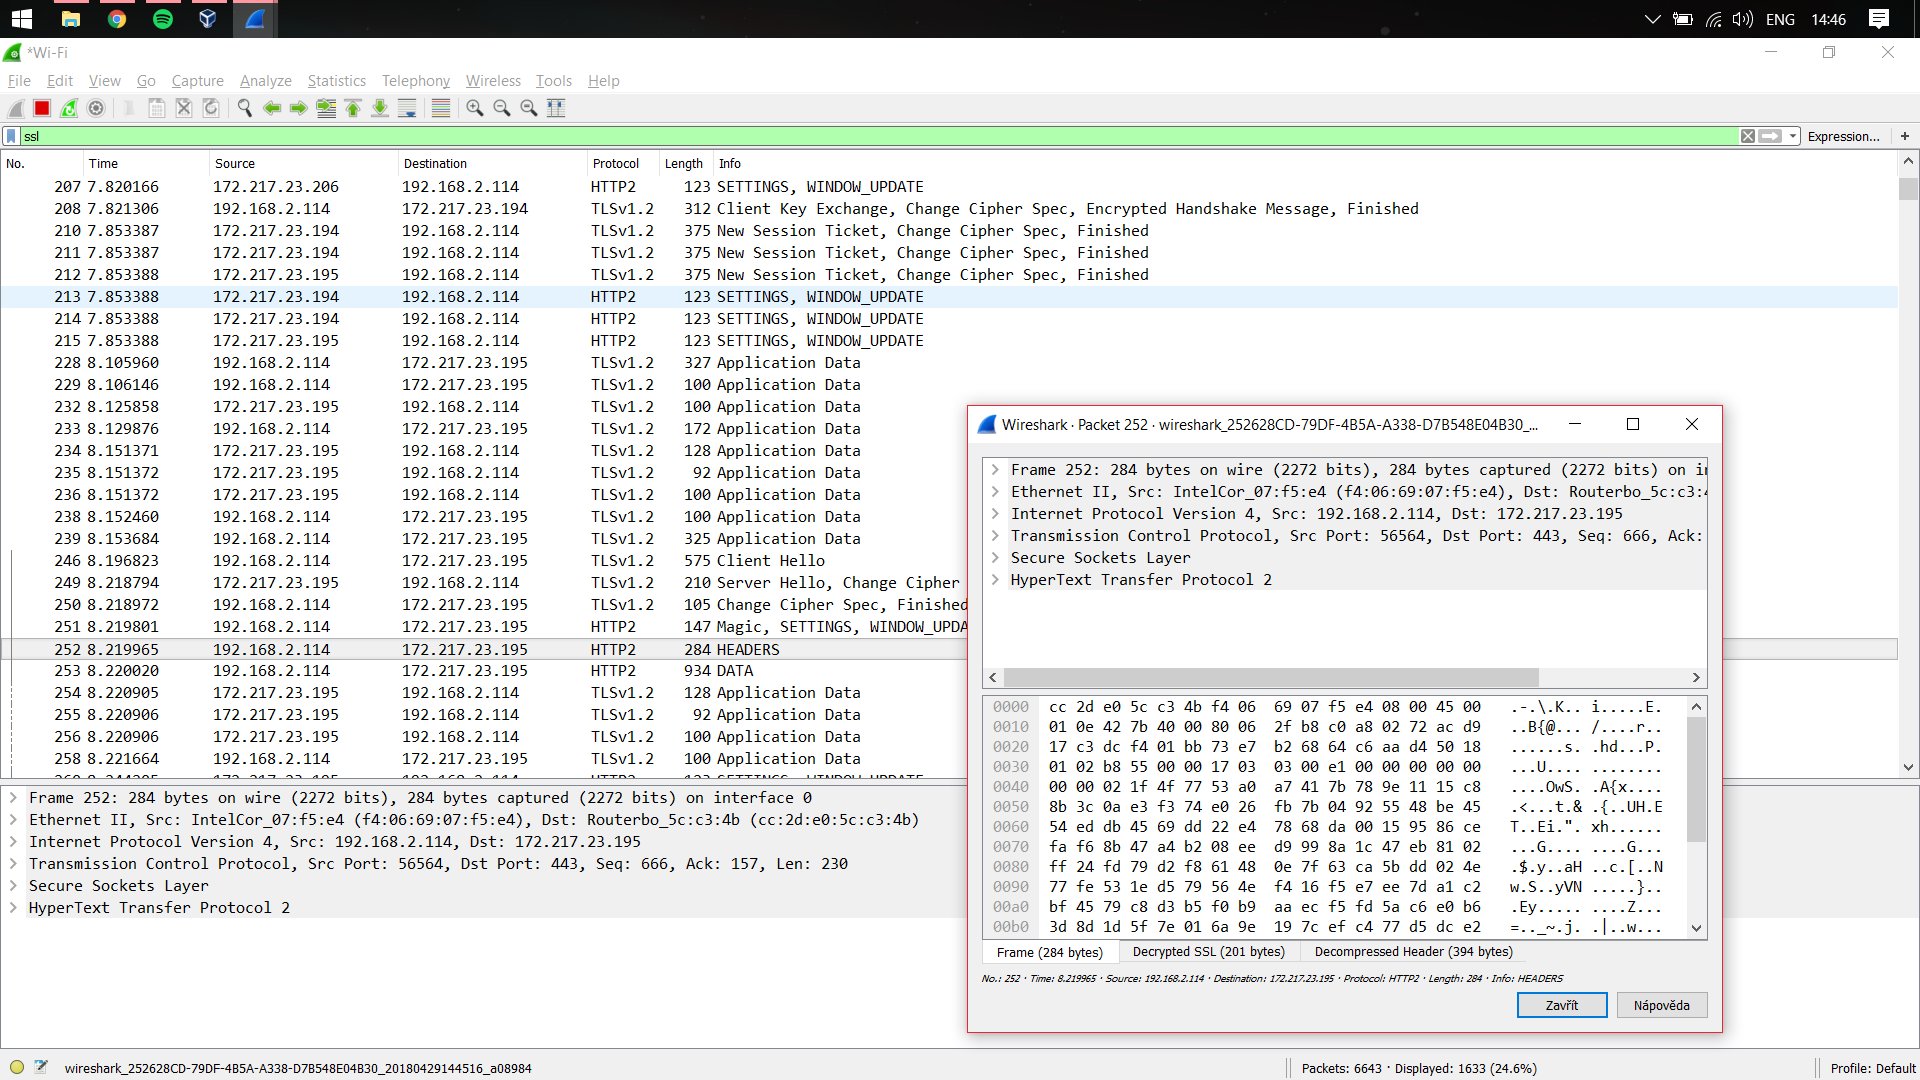
\includegraphics[width=0.8\textwidth]{encrypted.png}
      \caption{Zašifrovaný paket.\label{fig:encrypted}}
    \end{center}    
  \end{figure}

  \begin{figure}[h!]
    \begin{center}
      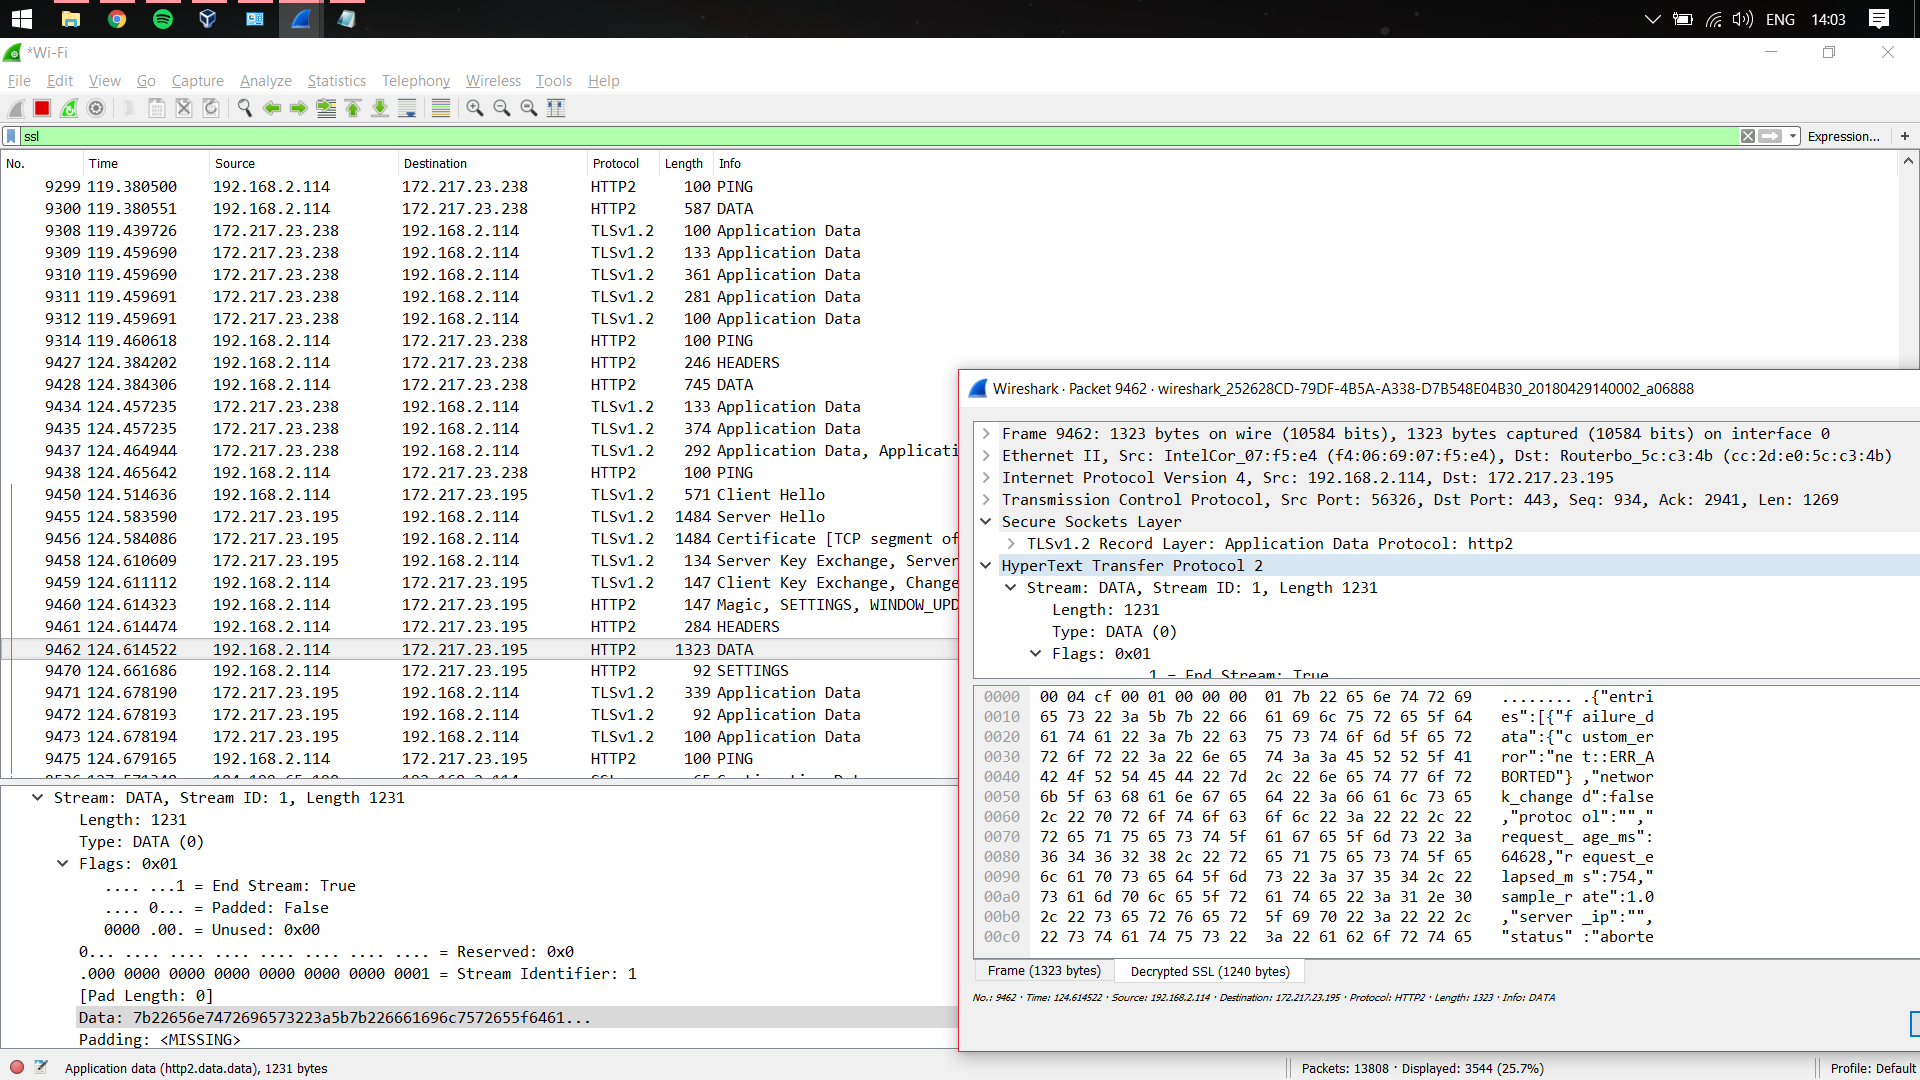
\includegraphics[width=0.8\textwidth]{decrypted.png}
      \caption{Dešifrovaný paket pomocí Wireshark.\label{fig:decrypted}}
    \end{center}    
  \end{figure}

  \section*{Zhodnocení výsledků}
  Při realizaci se povedlo dešifrovat odchozí a příchozí komunikaci. Takovýto
  útok by měl využití např. ve firemních sítích, nebo na veřejných počítačích (knihovny,
  internetové kavárny) pro kontrolu obsahu stránek, které jsou navštěvovány pro celkové
  zvýšení zabezpečení sítě, ať už z hlediska případného útoku (viry, trojské koně),
  nebo pro kontrolu obsahu jako takového (kyberkriminalita).

  Na druhou stranu takový útok je proveditelný pouze s patřičným oprávněním na dané stanici.
  Je nutné se tedy dostat k účtu, který daná práva má.
  
  % references
  \newpage
  \printbibliography

\end{document}